%==================================================================================================
%   LUKES THESIS TEMPLATE 1.2
%   -------------------------
%   This template is based upon the offcial IMM PhD Thesis template, it is enhanced with a number
%   of new features and a number of errors have fixed. This template is intended to be complied to
%   PDF using PDFLATEX and is tested using the MiKTeX 2.9 LaTeX distribution.
%   It is based on the official DTU-IMM Thesis template by Finn Kuno Christensen in 2009.
%   Small bugfixes by Kasper Laursen in 2012 and 2013.
%   Small updates by Finn Kuno Christensen/Henning Christiansen in 2015.
%   -------------------------
%   Last Updated: 2015-01-08
%==================================================================================================
%
%==================================================================================================
% DOCUMENT SETUP
%==================================================================================================
\documentclass[10pt,twoside]{book}                  %Official DTU-IMM Thesis document setup
%
%Set to 'print' for printed version, use 'net' for online version
\def\thesisversion{print}
%
%==================================================================================================
% PACKAGES
%==================================================================================================
\usepackage{LukeThesis}                             %Import Thesis base style
\usepackage{hyperref}
\usepackage{listings}
\usepackage{float}
\usepackage{tabularx}
\usepackage{tikz}
\usepackage{alltt}
\usepackage{todonotes}
\usepackage{url}
\usepackage{textcomp}
\usepackage{mathtools}
\usepackage{pdfpages}
\usepackage{amsmath}
\usepackage{framed}
\usetikzlibrary{positioning}
\usetikzlibrary{backgrounds}
\tikzstyle{every node}=[draw=black,thick,anchor=west]
%input{PhDMacros}                                   %Thesis specific macros
%
%==================================================================================================
% THESIS PROPERTIES (Modifiy these fields with your details)
%==================================================================================================
\def\thesisauthor{James Erik Groving Meade}                     %Author
\def\thesistitle{Hardware Accelerator for the Training of Neural Networks}               %Title
\def\thesishandin{28-June}                       %Submission date (Day-Month}
\def\thesisdegree{M.Sc.}                              %Degree ('B.Eng', 'B.Sc.', 'M.Sc.' or 'PhD')
\def\thesisyear{2019}                               %Submission year
\def\thesisnumber{????}                             %DTU-IMM Serial number (do not include year)
\def\thesisISSN{0000-0000}                          %ISSN number
\def\thesiskeywords{FPGA, Hardware, Computer Architecture, Neural Networks}  %PDF keywords
\derivethesisprops                                  %Derive dependent properties
%
%==================================================================================================
% SECTION NUMBERING SETUP
%==================================================================================================
\setcounter{tocdepth}{2}                            %2 adds sections up to subsections
\setcounter{secnumdepth}{3}                         %Subsubsections get a number when this is 3
%
%==================================================================================================
% THESIS STRUCTURE  (Modifiy to include more chapters etc)
%==================================================================================================
\definecolor{mygreen}{RGB}{28,172,0} 
\lstset{language=Verilog, 
	captionpos=b,
	basicstyle=\small\ttfamily,   
	breaklines=true,
	morekeywords={},
	keywordstyle=\color{blue},
	morekeywords=[2]{1}, keywordstyle=[2]{\color{black}},
	identifierstyle=\color{black},
	commentstyle=\color{mygreen},
	showstringspaces=false,
	frame=single,
	numbers=left,
	numberstyle={\small \color{black}},
	numbersep=9pt
}

\lstdefinelanguage{SystemVerilog}{
	keywords={always_ff, always_comb, if, begin, end, else, case, endcase, typedef, const, logic, integer, assign, parameter, localparam, module, posedge, negedge, enum, input, output},
	keywordstyle=\color{blue}\bfseries,
	ndkeywords={class, export, boolean, throw, implements, import, this},
	ndkeywordstyle=\color{darkgray}\bfseries,
	identifierstyle=\color{black},
	sensitive=false,
	comment=[l]{//},
	morecomment=[s]{/*}{*/},
	commentstyle=\color{mygreen}\ttfamily,
	stringstyle=\color{mygreen}\ttfamily,
	%morestring=[b]',
	morestring=[b]"
}



\tikzstyle{every node}=[draw=black,thick,anchor=west]
\begin{document}
%------------------------
%Pre-frontmatter material
%------------------------
\prefrontmatter
%--------------------
%Frontmatter material
%--------------------
\frontmatter
\pagenumbering{roman}                               %Set frontmatter numbering style
\chapter{Abstract}

The goal of the thesis is to ...                                   %English summary of Thesis
\markboth{}{}                                       %Set headings (left)(right)
%\input{SummaryDK}                                   %Danish summary of Thesis
%\markboth{}{}                                       %Set headings (left)(right)
\chapter{Preface}

This thesis was prepared at DTU Compute in fulfillment of the requirements for acquiring an M.Sc. in Computer Science and Engineering.

This thesis deals with the design of a hardware accelerator for the training of neural networks. Low-level design is one of my greatest passions and thus it has been an absolute privilege to have been given the opportunity to combine hardware with the surging field of machine learning. 

%==================================================================================================
% SIGNATURE AREA
%==================================================================================================
\vspace{20mm}
\begin{center}
    \hspace{20mm} Lyngby, \thesishandin-\thesisyear
    \vspace{5mm}
    \newline
  %Update signature image file in line below
    \includegraphics[scale=0.1]{figures/signature}
\end{center}
\begin{flushright}
    \thesisauthor
\end{flushright}
% % % EOF % % %                                     %Preface
\markboth{}{}                                       %Set headings (left)(right)
\chapter{Acknowledgements}

First and foremost, I would like to sincerely thank my advisor Jens Sparsø for his time and guidance throughout the entire duration of my thesis. Our regular meetings helped me to stay grounded and to think critically about my project.

I would also like to thank my former classmate, Cheng Fu, PhD student of the University of California, San Diego. My conversation with him at the beginning of my foray into the research literature helped me establish my footing.                            %Acknowledgements
\markboth{}{}                                       %Set headings (left)(right)
%------------------
% Table of contents
%------------------
\newpage\mbox{}\newpage
\chaptermark{Contents}
\pdfbookmark{\contentsname}{toc}
\renewcommand{\sectionmark}[1]{\markright{#1}}
\sectionmark{Contents}
\addtolength{\parskip}{-\baselineskip}
\tableofcontents
\addtolength{\parskip}{\baselineskip}
\renewcommand{\sectionmark}[1]{\markright{\thesection\ #1}}
%-------------
% Main content
%-------------
\mainmatter
\chapter{Introduction}
Neural networks have seen a surge in popularity ever since a neural network, coined AlexNet, decisively won the ImageNet Large Scale Visual Recognition Challenge in 2012, achieving 10.8\% higher accuracy then the next best solution \cite{Krizhevsky}. It was the only neural network entry in the entire competition; and the victory stunned much of the academic world.

This moment has been generally regarded as the spark that ignited the massive surge in academic interest toward neural networks and statistical machine learning. In the 7 years since, research regarding neural networks has yet to slow down as real-world applications of neural networks continue to be expand. To name a few examples, neural networks are currently in use for facial recognition at Facebook \cite{deepface}, translation for Microsoft \cite{translation}, spam filters for Google's Gmail \cite{gmail} and endless more.

In order for these neural networks to have such stellar accuracy on tasks such as image classification, they must first learn from labeled data in a process known as training. The neural network training process has an incredibly high level of inherent parallelism, and thus GPUs have emerged as the device of choice to train neural networks. GPU-based training takes advantage of data-level parallelism to train networks by assigning separate images in a training batch to different cores, which then all perform the same computations on different data. This coarsely-grained approach to training works well for large batch sizes. However, since these GPU models use data parallelism for speedup, GPU training models degrades for small batch sizes and are even slower than CPU models when it comes to online learning. Online learning is when a single labeled data sample is fed to the network at a time, or in other words, when the batch size is equal to 1 \cite{batch-size}. 

Today's solutions for training neural networks with small batch sizes do not take advantage of the fine-grain parallelism available in neural networks. This thesis presents a hardware accelerator that uses fine-grain parallelism at the neuron level to achieve high training performance. The accelerator results in much faster performance compared to the current solutions used by academia and industry when training neural networks with small batch sizes.

This thesis proposes a novel hardware architecture for the training of neural networks. While the focus of the thesis is the architectural design of the hardware accelerator, a basic understanding of neural networks is helpful. As such, Chapter \ref{background} reviews the basics of neural networks and surveys related work on designing hardware to optimize for neural network computation. Chapter \ref{ch-sw-model} describes the software model that was implemented to verify and further understand the algorithms to be used for the hardware model. Chapter \ref{hw-model} covers the hardware model and implementation of the accelerator. Next, Chapter \ref{hw-model-testing} documents the testing methods used to functionally verify the hardware model. Chapter \ref{results} presents the results of the thesis and Chapter \ref{analysis} provides analysis of these results. Chapter \ref{discussion} discusses the project as a whole and what future work could be done to improve the project. Finally, Chapter \ref{conclusion} presents the conclusion of the thesis.

                                  %Chapter 1
\chapter{Background and Motivation}
\section{A Brief Summary of Neural Networks}
\section{Related Work}                                 	%Chapter 2
\chapter{Software Model}
\label{ch-sw-model}
\todo[inline]{figure for code snippets or nah?}
\section{Overview}
This section documents the general-purpose neural network framework that was written in C++ for this thesis. There is an example program that trains on the MNIST dataset and documents epoch-by-epoch training statistics. MNIST is a dataset of handwritten digits, containing 60,000 training images and 10,000 test images. The source code for the software model can be found in the appendix as well as online on GitHub.\footnote{\url{
https://github.com/erikgroving/NeuralNetworkHardwareAccelerator/tree/master/SWModel}.}


\section{Motivation}
The software neural network framework was written so that the FPGA hardware model could be benchmarked against a CPU-based model that performs neural network inference and backward passes using the same method as the hardware model. This benchmark could be used to evaluate the performance of the hardware model. In addition, it could be benchmarked against professional open-source deep-learning frameworks that make use of advanced algebraic methods to perform computation such as matrix multiplication that inherently offer more efficiency. Furthermore, by developing a software model, the algorithmic integrity of the proposed network was able to verified and tested in an expedient manner by using a well-known testing framework, Google Test. Finally, if high floating-point precision were needed for training a network, then the software model could be used to learn the weights and parameters, and then subsequently be loaded into the weight BRAM of the FPGA hardware model.

\section{Design}
\subsection{Layers}
The software model was designed to be flexible such that any neural network architecture may be constructed so long as the layer types were implemented. The model currently supports 2D convolutional, fully connected, and pooling layers. 
\par 
All layers are derived from a base class, \texttt{Layer}. Certain methods such as \texttt{forward()} and \texttt{backward()} must be implemented by all derived classes. There is then a \texttt{Net} class that contains a \texttt{vector} of \texttt{Layer} objects. This allows for a flexible design, as one only need add layers to the \texttt{Net} object. Furthermore, the model can easily be extended to other layer types so long as the layer type derives from \texttt{Layer}. 
\par
The non-linear activation function used in the model is ReLU because the derivative is trivial to compute. Compared to the sigmoid function, ReLU is much more computationally feasible for an FPGA hardware implementation, and thereofre, ReLU was used in the software model so that both models would use the same activation function.
\subsection{Training}
\paragraph{The Softmax Function and Computing Loss Gradients}
The network uses an implicit Softmax function for the last layer since this converts the logits in the last layer to numbers that can be interpreted as probabilities, ideal for image classification. 
\par
The loss gradients for the neurons in the last layer are computed using multi-class cross entropy loss. Therefore, only one probability will account for loss, however, since each probability is an output from the softmax function which takes in all neuron outputs as input, all neurons in the last layer will have a loss gradient.
\par 
The derivative of this loss function is needed to perform backpropagation. We define $\mathcal{L}_i$ as the loss for neuron $i$ in the last layer and $z_i$ as the output of neuron $i$. We also introduce $y_i$, which is 1 if $x$ is an instance of class $i$ and 0 otherwise. We can then compute the loss gradient for neuron $i$ in the last layer quite simply as follows: 
\[    
\frac{\delta \mathcal{L}_i}{\delta z_i} = z_i - y_i
\]

\paragraph{Batch Size}
The software model supports batch training and thus a batch size is to be specified when creating an instance of a new network.
\paragraph{Learning Rate and Momentum}
The software model learns using stochastic gradient descent. As such, the network is configured with a learning rate and momentum. The learning rate may be manually readjusted during training epochs.



\section{Source Code Structure}
The software model contains a Makefile and three folders: \textit{data}, \textit{src} and \textit{test}. The \textit{data} folder contains the MNIST binary data files, and is loaded by the example program that trains on the MNIST dataset. The \textit{src} folder contains the source code of the neural network framework. The \textit{test} folder contains test made using the Google Test C++ testing framework. The Makefile is used to build the source as well as tests. This section will detail the source files in the \textit{src} folder that are core to the software model framework. The files \textit{main.cpp} and \textit{parse\_data\{.cpp, .h\}} will be described in section \ref{sw-usage} that focuses on usage.

\paragraph{net\{.cpp, .h\}}
These files contain the definition of the \texttt{Net} class, the highest-level class of the network. After initializing a \texttt{Net} object, layers can be added to the neural network by calling the \texttt{addLayer()} method which will add a \texttt{Layer} object to a \texttt{vector}. The \texttt{Net} class also stores intermediate activations from the current inference, which are required when performing backward pass to calculate loss gradients. The key parameters to the \texttt{Net} object are set in its constructor, and are defined in table \ref{nettable}. 
\begin{table}
	\centering
	\begin{tabularx}{\textwidth}{|l|l|X|}
		\hline
		\textbf{Name} 			& \textbf{Type} 		& \textbf{Description} \\\hline
		\texttt{in}  			& \texttt{uint32\_t}	& Size of the input to the neural network.\\\hline
		\texttt{out}			& \texttt{uint32\_t}	& Size of the output of the neural network. \\\hline 
		\texttt{bs}				& \texttt{uint32\_t}	& Size of the batch size to be used when training the net.\\\hline 
		\texttt{lr}				& \texttt{double}	& The learning rate to be used during training of the network. Can be set and read using the functions \texttt{setLearningRate()} and \texttt{getLearningRate()}. \\\hline 
		\texttt{momentum}		& \texttt{double}	& The momentum to be used when performing updates to the weights and biases of the network.
		\\\hline
	\end{tabularx}
	\caption{Description of parameters for the constructor \texttt{Net} class.}
	\label{nettable}
\end{table}
\par 
The \texttt{Net} class has a method \texttt{inference()} that computes the forward pass for a batch of inputs, thus the argument is a 2-d \texttt{vector}, with each outer index corresponding to an input. The \texttt{()} operator has also been overloaded to call \texttt{inference()}. This is all that is needed to compute a forward pass.
\par 
To compute the backward pass, \texttt{computeLossAndGradients()} should be called first. This method takes in the label data as a \texttt{vector} for the inputs as an argument and computes the loss gradients for the outer layer of the network. Next, a call to \texttt{backpropLoss()} should be made; this method propagates the outer layer loss gradients back through the neural network. After the loss has been back-propagated, weights of each \texttt{Neuron} in the network should be updated by calling \texttt{update()}. Previously cached forward pass activation data should then be cleared with a call to \texttt{clearSavedData()}.
\paragraph{layer.h}
This file contains the \texttt{Layer} class, which serves as the base class for all the different types of layer classes in the framework. It contains virtual methods \texttt{forward()} and \texttt{backward()}, representing the forward and backward pass functionality that must be implemented. All layer classes must also contain a \texttt{getType()} method to identify the layer type, as well as methods for \texttt{updateWeights()}, \texttt{clearData()}, and \texttt{getOutput()}.

\paragraph{convolutional\{.cpp, .h\}}
These files contain the definition of the \texttt{ConvLayer} class, which implements a 2D-convolutional layer, and derives from the \texttt{Layer} class. A unique method to the \texttt{ConvLayer} class is the \texttt{getWindowPixels()} method, which returns the pixels inside the filter window, and is used when computing both the forward and backward passes.  The class' constructor and key parameters are described in table \ref{convtable}.
\begin{table}
\centering
\begin{tabularx}{\textwidth}{|l|l|X|}
	\hline
	\textbf{Name} 			& \textbf{Type} 		& \textbf{Description} \\\hline
	\texttt{dim}  			& \texttt{uint32\_t}	& Dimensions of the input. The dimension is assumed square, meaning that rows = \texttt{dim} and columns = \texttt{dim}.\\\hline
	\texttt{filt\_size} 	& \texttt{uint32\_t}	& Dimension of the filter used for the convolution, dimension also assumed square. \\\hline 
		\texttt{stride} 	& \texttt{uint32\_t}	& Size of the stride \\\hline 
	\texttt{padding} 		& \texttt{uint32\_t}	& Padding used for convolution. \\\hline 
	\texttt{in\_channels} 	& \texttt{uint32\_t}	& Amount of channels in the input. \\\hline 
	\texttt{out\_channels} 	& \texttt{uint32\_t}	& Amount of channels in the output. \\\hline
\end{tabularx}
\caption{Description of parameters for the \texttt{ConvLayer} class.}
\label{convtable}
\end{table}


\paragraph{fullyconnected\{.cpp,.h\}}
These files define the \texttt{FullyConnected} class. The class only has two defining parameters in its constructor: \texttt{in} and \texttt{out}, which are of type \texttt{uint32\_t} and specify the input and output size to the layer, respectively. It derives from the base \texttt{Layer} class, so methods such as \texttt{forward()} and \texttt{backward()} are also implemented.

\paragraph{pooling\{.cpp,.h\}}
These files define the \texttt{PoolingLayer} class. The class derives from \texttt{Layer} and performs a 2D 2$\times$2 max pooling operation. There are three main parameters for the class: \texttt{dim\_i}, \texttt{dim\_o}, and \texttt{channels}. The parameters \texttt{dim\_i} and \texttt{dim\_o} specify the dimension of the input and output feature vectors. Since the layer currently only performs 2$\times$2 max pooling, \texttt{dim\_o} will always be half of \texttt{dim\_i}, though if different types of pooling filters were to be supported, then \texttt{dim\_o} would be necessary. The \texttt{channels} parameter is used to specify the number of channels of size \texttt{dim\_i} $\times$ \texttt{dim\_i} present in the input.

\paragraph{neuron\{.cpp, .h\}}
These files define the \texttt{Neuron} class. The \texttt{Neuron} class is the computational building block of the fully connected and convolutional layers. The fan-in of the neuron is specified in the constructor. Weights should be initialized using the \texttt{initWeights()} method, which implements He initialization \cite{HeZR015}. He initialization randomly initializes weights using a normal distribution with a mean of 0 and a variance of $\frac{2}{\text{fan\_in}}$. 
\par 
The class implements all necessary computational elements for a neuron in a neural network. During a forward pass, a neuron's net and activation are computed with \texttt{computeNet()} and \texttt{computeActivation()} respectively. When computing the backward pass, the gradients for the neuron's weights are computed using \texttt{calculateGradient()}. Weights can be subsequently updated using the \texttt{updateWeights()} function. Finally, all gradient data can be cleared using \texttt{clearBackwardData()}.

\section{Usage}\label{sw-usage}
This section will show how the software model may be used for image classification. In the following example, the software model will be trained to classify handwritten digits from the MNIST database. Each image is a handwritten digit of size 28$\times$28. The relevant files specific to this example are \textit{main.cpp} and \textit{parse\_data.cpp}.
\paragraph{Load the Training and Testing Data}
The first step to any neural network problem is to load the training and testing dataset.
The MNIST dataset is provided as binary files and helper functions to load the data have been provided in \textit{parse\_data.cpp}. Training and testing data can be loaded as shown below.
\begin{lstlisting}[language=c++]
std::vector< std::vector<double> > trainX;
std::vector<int> trainY;
std::vector< std::vector<double> > testX;
std::vector<int> testY;
trainX = readImages("data/train-images.idx3-ubyte");
trainY = readLabels("data/train-labels.idx1-ubyte");
testX = readImages("data/t10k-images.idx3-ubyte");
testY = readLabels("data/t10k-labels.idx1-ubyte");
\end{lstlisting}
\paragraph{Create a \texttt{Net} Instance}
The next step is to create a \texttt{Net} object with the relevant hyperparameters to be used for the neural network. The below code accomplishes this.
\begin{lstlisting}[language=c++]
int 	input_size  = 28*28;
int     output_size = 10;
int     batch_size  = 200;
double  momentum    = 0.9;
double  lr          = 0.01; 
Net net(input_size, output_size, batch_size, lr, momentum);
\end{lstlisting}

\paragraph{Create Layer Objects and Add them to the \texttt{Net} Object} 
After the \texttt{Net} object has been created, layers need to be added to the network. Two configuration options are present in \textit{main.cpp}; one implements a 7-layer convolutional neural network, and the other implements a 4-layer fully connected neural network. The below code snippet shows how the 7-layer convolutional neural network is implemented. The software model was designed with simplicity in mind, so the below code is relatively straightforward to follow.
\begin{lstlisting}[language=c++]
Layer* conv1 = new ConvLayer(28, 3, 1, 1, 1, 8);
Layer* pool1 = new PoolingLayer(28, 14, 8);
Layer* conv2 = new ConvLayer(14, 3, 1, 1, 8, 16);
Layer* pool2 = new PoolingLayer(14, 7, 16);
Layer* fc1 = new FullyConnected(16*7*7, 64);
Layer* fc2 = new FullyConnected(64, 10);

net.addLayer(conv1);
net.addLayer(pool1);
net.addLayer(conv2);
net.addLayer(pool2);
net.addLayer(fc1);
net.addLayer(fc2);
\end{lstlisting}

\paragraph{Train the Net}
In \textit{main.cpp}, a function \texttt{trainNet()} has been implemented, which trains the net using batch training. The actual training for a given batch only requires 5 lines of code, and is shown below.
\begin{lstlisting}[language=c++]
net(in_batch);
net.computeLossAndGradients(out_batch);
net.backpropLoss();
net.update();
net.clearSavedData();
\end{lstlisting}
\paragraph{Build and Run the Model}
Compile the code by running \texttt{make} in the \textit{SWModel} directory. The model will then train for the amount of epochs specified in the call to the \texttt{trainNet()} function in \texttt{main()}. Since the model is initialized with random weights, the final result of training is non-deterministic. Output similar to the output shown in figure \ref{sw-model-output} can be expected. In this case, the fully connected model was used, and train to a maximum accuracy of 97.62\%. it is also worth noting the expected differences in loss and accuracy between the training and test datasets. This discrepancy is expected as the network never learns from the test dataset.
The difference between test and training dataset accuracy is normally used to quantify how well the network is able to generalize from the training dataset.
\begin{figure}
\begin{lstlisting}
Running software model...
Starting Accuracy
Total correct: 1022 / 10000
Accuracy: 0.1022

Epoch: 0
--- Training Stats ---
Total correct: 54914 / 60000
Accuracy: 0.915233
Loss: 0.290908
--- Test Stats ---
Total correct: 9183 / 10000
Accuracy: 0.9183
Loss: 0.280574

Epoch: 1
--- Training Stats ---
Total correct: 56213 / 60000
Accuracy: 0.936883
Loss: 0.218062
--- Test Stats ---
Total correct: 9390 / 10000
Accuracy: 0.939
Loss: 0.214584

...

Epoch: 36
--- Training Stats ---
Total correct: 59168 / 60000
Accuracy: 0.986133
Loss: 0.0516957
--- Test Stats ---
Total correct: 9762 / 10000
Accuracy: 0.9762
Loss: 0.0845137
\end{lstlisting}
\caption{An expected output from using the software model on the provided MNIST dataset. Epochs 2-35 omitted for brevity. In this training run, the network reached a maximum test set accuracy of 97.62\%.}
\label{sw-model-output}
\end{figure}

\section{Testing}
To ensure the correctness of the software model, several test suites were created during development. Source code for the test suites can be found in the \textit{test} folder as well as in the appendix.
\todo[inline]{source code in appendix}
\subsection{Test Suites}
Four test suites were created during the development of the software model. The test cases were written to test features as they were developed. As such, the tests include neuron functionality, forward pass for fully connected and convolutional layers, and finally a gradient checking test suite to verify the backward pass. This section elaborates on the test suites that were used during development.

\paragraph{Neuron Testing}
The neuron test suite, found in \textit{neuron\_test.cpp}, contains one primary test case that sets the weights of a neuron, computes the activation, and verifies that the activation is correct.

\paragraph{Fully Connnected Forward Pass}
The test case for a fully connected layer's forward pass is located in \textit{fullyconnected\_test.cpp}. The test case creates a \texttt{FullyConnected} layer that has 3 inputs and 4 outputs. The weights are then set and an input is sent forward through the layer. Each of the 4 outputs are then verified to be correct.

\paragraph{Convolutional Forward Pass}
There is a test case to verify the convolutional forward pass located in \textit{conv\_test.cpp}. The test creates a convolutional layer that takes a 2$\times$2 feature vector with 2 channels, uses a 3$\times$3 filter for convolution, uses a stride and padding of 1, and produces 2 output channels. Weights and inputs were the arbitrarily assigned and the forward pass was computed and verified against the output that had been previously calculated manually.

\paragraph{Gradient Checking}
It would be very tedious and error-prone to debug the backward pass of a neural network using manual calculations, thus the general standard method of testing the gradients computed during a backward pass is to use gradient checking. Note that during the backward pass, all the loss gradients for every single weight and bias are calculated. For every weight (and bias), the partial derivative $\frac{\delta \mathcal{L}}{\delta w_i}$ is computed. Gradient checking verifies that the mathematically computed analytic derivative aligns with a numerically estimated derivative \cite{grad-check-stanford}. The numerical gradient can be computed as follows:
\begin{align*}
	\frac{\delta \mathcal{L}(w_i)}{\delta w_i} = \frac{\mathcal{L}(w_i + \epsilon) - \mathcal{L}(w_i - \epsilon)}{2\epsilon}
\end{align*}
The partial derivative of the loss with respect to a certain weight $w_i$ can thus be estimated by calculating the loss after incrementing $w_i$ by a small $\epsilon$, calculating the loss after decrementing $w_i$ by $\epsilon$, and then dividing the difference by $2\epsilon$. As long as $\epsilon$ is rather small, the derivatives should be near exact. In these test cases, $\epsilon = 10^{-4}$. Once we have the analytic and numerical gradient, we can compute the relative error as shown below:
\begin{align*}
	\text{Relative gradient error} = \frac{\lvert\mathcal{L}'(w_i)_a - \mathcal{L}'(w_i)_n\rvert}
		{\max \;\left(\lvert\mathcal{L}'(w_i)_a\rvert,\; \lvert\mathcal{L}'(w_i)_n\rvert\right)}
\end{align*}
If the relative error is below a certain threshhold, then it is safe to assume the gradient has been calculated correctly. In this test suite, the relative error threshhold must be lower than $10^{-7}$.
\par 
The two test cases in \textit{gradient\_check\_test.cpp} perform gradient checks for a fully connected network and for a convolutional neural network. The fully connected network gradient check test creates a neural network with an architecture shown in figure \ref{fctest}.
\begin{figure}
	\begin{lstlisting}[language=C++]
int 	input_size  = 100;
int 	output_size = 2;
int 	batch_size  = 1;
double 	momentum    = 0.9;
double 	lr          = 0.001; 
Net net(input_size, output_size, batch_size, lr, momentum);


Layer* fc1 = new FullyConnected(input_size, 98);
Layer* fc2 = new FullyConnected(98, 64);
Layer* fc3 = new FullyConnected(64, output_size);

net.addLayer(fc1);
net.addLayer(fc2);
net.addLayer(fc3);		
	\end{lstlisting}
	\caption{Layer created for the fully connected gradient check test.}
	\label{fctest}
\end{figure}
\par
The test then creates 10 random inputs, each having a random label. Each input sample is fed forward through the network and analytic gradients are computed for each weight. The numerical gradient is then subsequently computed for a random weight. The random weight can belong to any neuron and any layer. This process of choosing a random weight, calculating the numerical gradient, comparing it to the analytic gradient is then repeated 100 times. The test asserts that the relative error is less than $10^{-7}$ each time. A portion of the computed analytic and numerical gradients are shown in figure \ref{num-grads}.
\begin{figure}
	\begin{lstlisting}
Layer: 2, Neuron: 0,  Weight: 31 
Analytic Gradient: -0.0638284 Numerical Gradient: -0.0638284

Layer: 0, Neuron: 93, Weight: 71 
Analytic Gradient: -0.156235  Numerical Gradient: -0.156235

Layer: 1, Neuron: 34, Weight: 29 
Analytic Gradient: -1.22615   Numerical Gradient: -1.22615

Layer: 1, Neuron: 12, Weight: 43 
Analytic Gradient: 0.376021   Numerical Gradient: 0.376021		
	\end{lstlisting}
	\caption{Results from the fully connected test using randomly sampled weights to perform gradient checking}
	\label{num-grads}
\end{figure}

The convolutional gradient checking test is set up in the same manner as the fully connected gradient checking test, except that the network structure is different. The network is now a \textbf{convolutional layer --- pooling layer --- convolutional layer --- fully connected layer}. The input is randomized 8x8 data, and convolutional layers use 3$\times$3 filters with a padding and stride set to 1. The first convolutional layer has 3 output channels and the second convolutional layer has 3 input channels and 6 output channels. The code used to create the network is shown in figure \ref{conv-net}.

\begin{figure}
	\begin{lstlisting}[language=C++]
int    input_size   = 8*8;
int    output_size  = 2;
int    batch_size   = 1;
double momentum     = 0.9;
double lr           = 0.001; 
Net net(input_size, output_size, batch_size, lr, momentum);

Layer* conv1 = new ConvLayer(8, 3, 1, 1, 1, 3);
Layer* pool1 = new PoolingLayer(8, 4, 3);
Layer* conv2 = new ConvLayer(4, 3, 1, 1, 3, 6);
Layer* fc1   = new FullyConnected(4*4*6, output_size);

net.addLayer(conv1);
net.addLayer(pool1);
net.addLayer(conv2);
net.addLayer(fc1);	
	\end{lstlisting}
	\caption{Layer created for the convolutional layer gradient check test.}
	\label{conv-net}
\end{figure}


\subsection{Building and Running the Test Suites}
The test suites requires Google Test to compile. Google Test can be downloaded online at GitHub \footnote{\url{https://github.com/google/googletest}}. The \textit{googletest} directory should then be placed under the \textit{SWModel} folder. The test suite can then be compiled using the provided Makefile and the following command:
\begin{lstlisting}
> make all_tests
\end{lstlisting}
This will produce an executable in the \textit{SWModel} directory called \textbf{all\_tests}. The test suites can be run by invoking the executable. The output is shown in figure \ref{goog-out}
\begin{figure}

\begin{framed}
\begin{alltt}
> ./all\_tests
Running main() from ./googletest/src/gtest\_main.cc
{\color{mygreen}[==========]} Running 6 tests from 4 test cases.
{\color{mygreen}[----------]} Global test environment set-up.
{\color{mygreen}[----------]} 1 test from ConvTest
{\color{mygreen}[ RUN      ]} ConvTest.TestForward
{\color{mygreen}[       OK ]} ConvTest.TestForward (1 ms)
{\color{mygreen}[----------]} 1 test from ConvTest (11 ms total)

{\color{mygreen}[----------]} 1 test from FCTest
{\color{mygreen}[ RUN      ]} FCTest.TestForward
{\color{mygreen}[       OK ]} FCTest.TestForward (0 ms)
{\color{mygreen}[----------]} 1 test from FCTest (10 ms total)

{\color{mygreen}[----------]} 2 tests from NeuronTest
{\color{mygreen}[ RUN      ]} NeuronTest.InitWeights
{\color{mygreen}[       OK ]} NeuronTest.InitWeights (0 ms)
{\color{mygreen}[ RUN      ]} NeuronTest.SetWeightsAndGetOutput
{\color{mygreen}[       OK ]} NeuronTest.SetWeightsAndGetOutput (0 ms)
{\color{mygreen}[----------]} 2 tests from NeuronTest (29 ms total)

{\color{mygreen}[----------]} 2 tests from GradientTest
{\color{mygreen}[ RUN      ]} GradientTest.FCGradientCheck
{\color{mygreen}[       OK ]} GradientTest.FCGradientCheck (950 ms)
{\color{mygreen}[ RUN      ]} GradientTest.ConvGradientCheck
{\color{mygreen}[       OK ]} GradientTest.ConvGradientCheck (2260 ms)
{\color{mygreen}[----------]} 2 tests from GradientTest (3223 ms total)

{\color{mygreen}[----------]} Global test environment tear-down
{\color{mygreen}[==========]} 6 tests from 4 test cases ran. (3329 ms total)
{\color{mygreen}[  PASSED  ]} 6 tests.
\end{alltt}
\end{framed}
\caption{Test coverage output using the Google Test C++ testing framework to verify the correctness of the software model for both forward and backward passes.}
\label{goog-out}
\end{figure}

                                  %Chapter 3
\chapter{Hardware Model and Implementation}                                  %Chapter 4
\chapter{Hardware Model Testing and Verification}
\section{Simulation}
\section{MMIO}
                                  %Chapter 5
\chapter{Results}\label{results}
Some of the results in this chapter are based on evaluating the hardware model (HWM) against other models implementing the same neural network. The other models include my software model (SWM), PyTorch running on the CPU (PyCPU), and PyTorch running on the GPU (PyGPU). My software model performs the same computations as the hardware model, so this provides insight to speedup over CPU without computational optimizations. The PyTorch CPU and GPU models then compare my hardware accelerator against heavily-optimized neural network frameworks. A training epoch in the following experiments is defined as performing learning on the 60,000 training images of the MNIST dataset. Inference experiments measure time to perform inference on all 70,000 images in the MNIST dataset.

\todo[inline]{runtime not speedup/eff}
Figures \ref{gpu-speedup} and \ref{gpu-eff} show PyGPU speedup and efficiency for varying batch sizes, respectively. As one might notice, there is no degradation in efficiency whatsoever. In fact, there are efficiencies even higher than 1. For batch size, this is plausible because increasing the batch size will slightly decrease the amount of work needed to be performed. The amount of forward and backward passes remains the same, though only 1 update of the weights needs to be performed for each batch. This means that a batch size of 1 performs 5 times more weight updates than a batch size of 5, which performs 20 times more weight updates than a batch size of 100. Therefore it is for this reason that efficiency remains around 1 even with massive batch sizes. Ultimately, it shows the massive amount of parallelism present in the training of neural networks. 

From the figures, it is clear that the GPU model takes advantage of data-level parallelism to achieve performance, as epoch time is a near linear function of batch size. As a result, since the GPU-based implementation uses a coarser form of parallelism compared to the HWM, it would be illogical to benchmark speedup against the GPU with a batch size of 1. Therefore, the PyGPU model has been benchmarked using a batch size of 50 unless otherwise specified. It should be noted that the PyGPU model also performs 49 fewer weight updates as a result of this. Moreover, each weight update on a GPU would require reductions of partial gradient results from the CUDA kernels, so this should be taken into consideration when observing the following performance benchmarks.

\begin{figure}
	\centering
	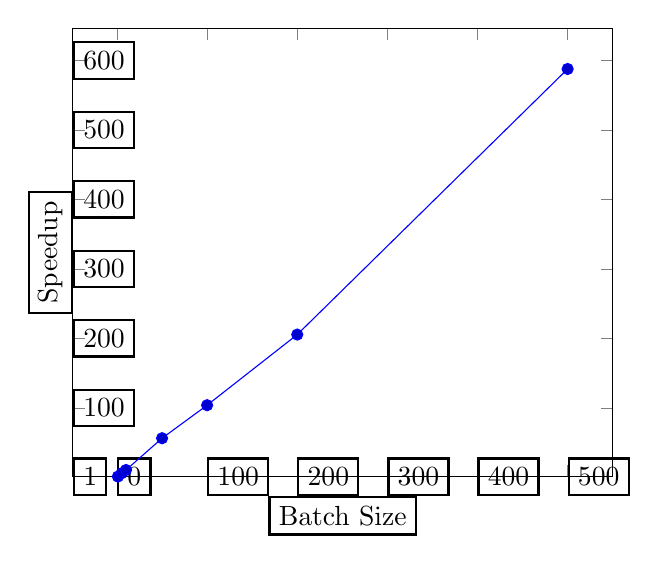
\begin{tikzpicture}
	\begin{axis}
	[ymin=1, ytick = {1, 100, 200, 300, 400, 500, 600}, ylabel={Speedup}, xlabel={Batch Size}]
	\addplot coordinates 
	{(1,1) (5, 5.59) (10, 10.436) (50, 56.178) (100, 103.73) (200, 205.404) (500, 587.764)};
	\end{axis}
	\end{tikzpicture}
	\caption{GPU speedup by increasing batch size}
	\label{gpu-speedup}
\end{figure}

\begin{figure}
	\centering
	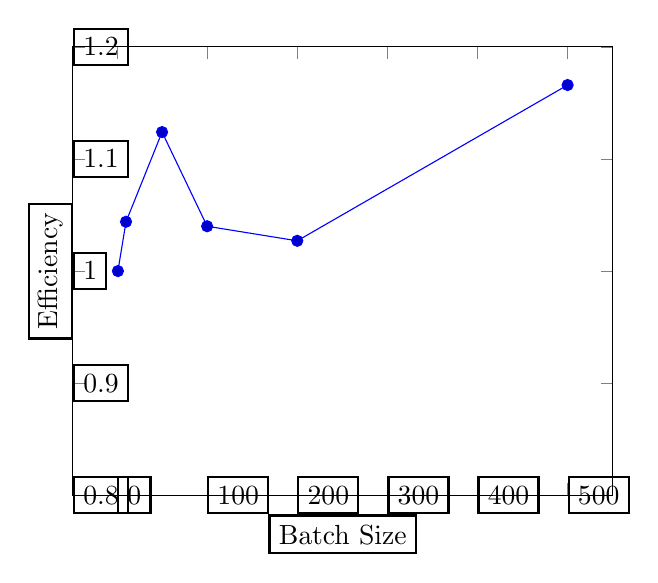
\begin{tikzpicture}
	\begin{axis}[
	ymin=0.8, ymax = 1.2, ylabel={Efficiency}, xlabel={Batch Size}]
	\addplot coordinates 
	{(1,1) (10, 1.044) (50, 1.124) (100, 1.04) (200, 1.027) (500, 1.166)};
	\end{axis}
	\end{tikzpicture}
	\caption{GPU efficiency by increasing batch size}
	\label{gpu-eff}
\end{figure}

\section{Evaluation Hardware}
The hardware model is evaluated using a ZedBoard equipped with a Zynq-7000 XC7Z020 SoC. The SWM and PyCPU both run on a Intel Core i7-4720HQ CPU. The GPU is an Nvidia GeForce GTX 970M equipped with 6 GB of GDDR5 RAM.

\section{Performance}
One of the most important metrics for an accelerator is runtime performance. 
While this hardware model is primarily focused on training, experiments to determine performance for both training and inference modes have both been conducted and are shown in this section.

\subsection{Training}
The average time for 1 training epoch has been recorded for each of the neural network models. The result is shown in Figure \ref{train-runtime-res}. This graph shows that the accelerator massively outperforms CPU models. Figure \ref{train-speedup-res} shows the speedup of the models, using PyCPU as a baseline. Notably, the HWM achieves a speedup of of nearly equal to that of the PyGPU model.

\begin{figure}
	\centering
	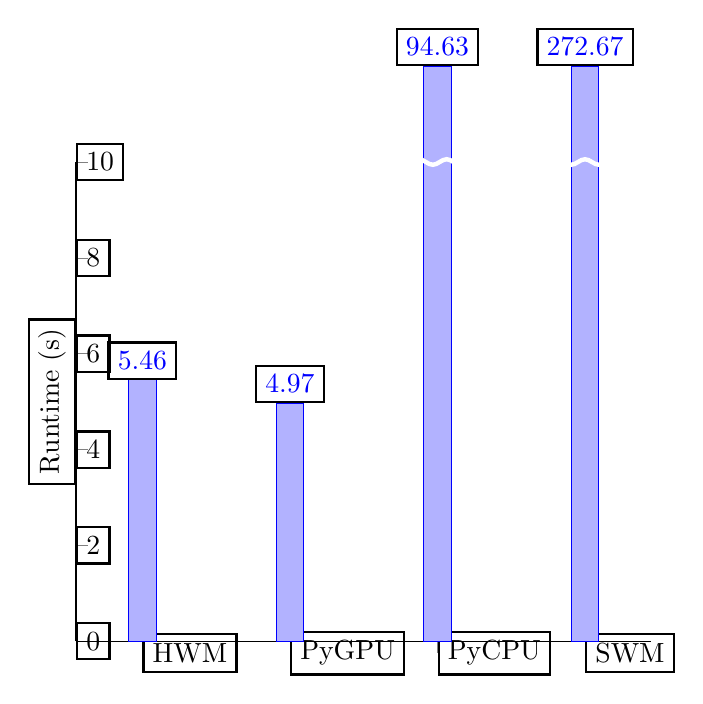
\begin{tikzpicture}
	\begin{axis}[
	ybar,
	width=3.5in,
	enlarge y limits=false,
	enlarge x limits=0.15,
	legend style={at={(0.5,-0.15)},
		anchor=north,legend columns=-1},
	ylabel={Runtime (s)},
	ymin=0,
	ymax=10,
	xmax=SWM,
	restrict y to domain*=0:12, % Cut values off at 14
	visualization depends on=rawy\as\rawy, % Save the unclipped values
	after end axis/.code={ % Draw line indicating break
		\draw [ultra thick, white, decoration={snake, amplitude=1pt}, decorate] (rel axis cs:0.1,1.0) -- (rel axis cs:1.0,1.0);},
	axis lines*=left,
	clip=false,
	nodes near coords={{\pgfmathprintnumber{\rawy}}},
	symbolic x coords={HWM, PyGPU, PyCPU, SWM},
	xtick={data}
	]
	
	\addplot coordinates {(HWM, 5.455)  (PyGPU, 4.9689) (PyCPU, 94.633) (SWM, 272.67)};
	
	\end{axis}
	\end{tikzpicture}
	\caption{Training runtime for various network models}
	\label{train-runtime-res}
\end{figure}

\begin{figure}
	\centering
	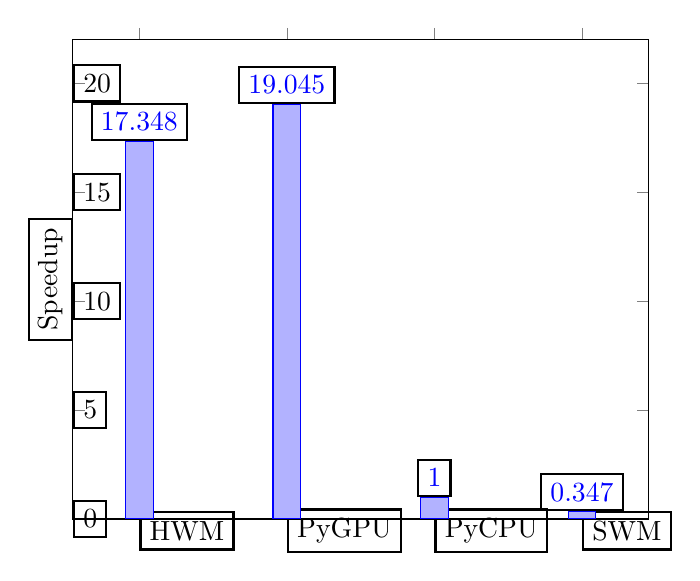
\begin{tikzpicture}
	\begin{axis}[
	ybar,
	width=3.5in,
	enlarge y limits=false,
	enlarge x limits=0.15,
	legend style={at={(0.5,-0.15)},
		anchor=north,legend columns=-1},
	ylabel={Speedup},
	ymin=0,
	ymax=22,
	xmin=HWM,
	xmax=SWM,
	symbolic x coords={HWM, PyGPU, PyCPU, SWM},
	xtick={data},
	scaled y ticks=false,
	nodes near coords,
	nodes near coords style={/pgf/number format/fixed},	
	nodes near coords style={/pgf/number format/precision=3},
	nodes near coords align={vertical}
	]
	
	\addplot coordinates {(HWM, 17.348)  (PyGPU, 19.045) (PyCPU, 1) (SWM, 0.347)};
	
	\end{axis}
	\end{tikzpicture}
	\caption{Training speedup using the PyCPU as a baseline}
	\label{train-speedup-res}
\end{figure}


\subsection{Inference}
Inference performance was also measured for each of the models. The result is shown in Figure \ref{inf-runtime-res}. This graph shows that the accelerator also outperforms CPU models for inference, though falls short of the GPU model. Figure \ref{inf-speedup-res} shows the speedup of the models, using PyCPU as a baseline. The HWM achieves a speedup of 2.282 compared to the PyCPU model.

\begin{figure}
	\centering
	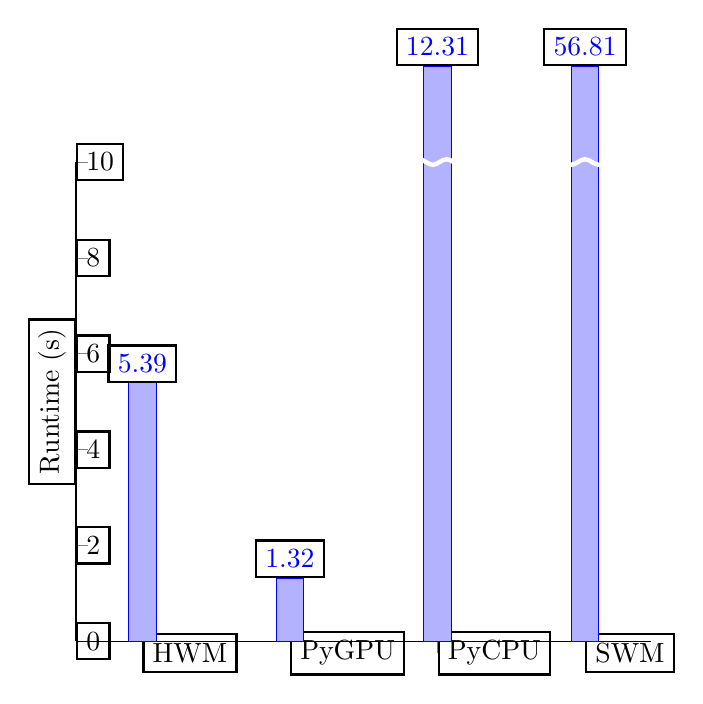
\begin{tikzpicture}
	\begin{axis}[
	ybar,
	width=3.5in,
	enlarge y limits=false,
	enlarge x limits=0.15,
	legend style={at={(0.5,-0.15)},
		anchor=north,legend columns=-1},
	ylabel={Runtime (s)},
	ymin=0,
	ymax=10,
	xmax=SWM,
	restrict y to domain*=0:12, % Cut values off at 14
	visualization depends on=rawy\as\rawy, % Save the unclipped values
	after end axis/.code={ % Draw line indicating break
		\draw [ultra thick, white, decoration={snake, amplitude=1pt}, decorate] (rel axis cs:0.1,1.0) -- (rel axis cs:1.0,1.0);},
	axis lines*=left,
	clip=false,
	symbolic x coords={HWM, PyGPU, PyCPU, SWM}, 
	nodes near coords={{\pgfmathprintnumber{\rawy}}},
	xtick={data}
	]
	
	\addplot 
	coordinates {(HWM, 5.392)  (PyGPU, 1.32) (PyCPU, 12.305) (SWM, 56.808)};
	
	\end{axis}
	\end{tikzpicture}
	\caption{Inference runtime for various network models}
	\label{inf-runtime-res}
\end{figure}

\begin{figure}
	\centering
	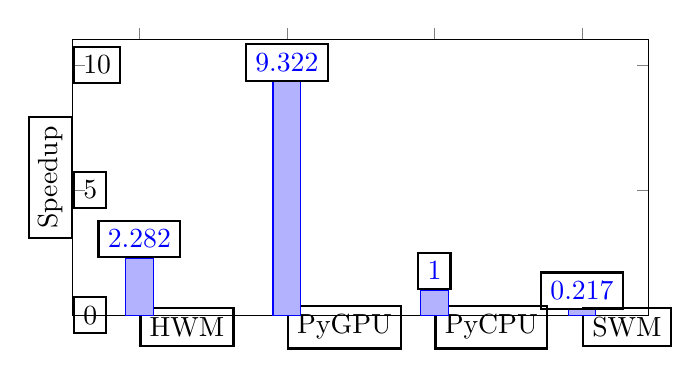
\begin{tikzpicture}
	\begin{axis}[
	ybar,
	height=2in,
	width=3.5in,
	enlarge y limits=false,
	enlarge x limits=0.15,
	legend style={at={(0.5,-0.15)},
		anchor=north,legend columns=-1},
	ylabel={Speedup},
	ymin=0,
	ymax=11,
	xmin=HWM,
	xmax=SWM,
	symbolic x coords={HWM, PyGPU, PyCPU, SWM},
	xtick={data},
	scaled y ticks=false,
	nodes near coords,
	nodes near coords style={/pgf/number format/fixed},	
	nodes near coords style={/pgf/number format/precision=3},
	nodes near coords align={vertical}
	]
	
	\addplot coordinates {(HWM, 2.282)  (PyGPU, 9.322) (PyCPU, 1) (SWM, 0.217)};
	
	\end{axis}
	\end{tikzpicture}
	\caption{Inference speedup using the PyCPU as a baseline}
	\label{inf-speedup-res}
\end{figure}

\subsection{Active/Idle Cycles}
To determine the impact of using MMIO via AXI bus to transfer image data between the PS and the FPGA, active and idle cycles were measured during training and inference. An active cycle is defined as a cycle on the FPGA during which at least one of the layers was computationally active. An idle cycle is thus defined as a non-active cycle. 

An experiment was performed to measure active cycle percentages for the HWM during inference and training. The dataset was the entire MNIST dataset in both cases. The active cycle percentage for inference and training are shown in Table \ref{active-cycle-table}.

\begin{table}
	\centering 
	\begin{tabular}{|c|c|}
		\hline
		& \textbf{Active Cycle Percentage} \\\hline
		Inference & 25.13\% \\\hline 
		Training & 69.20\% \\\hline
	\end{tabular}
	\caption{Active Cycle Percentages for inference and training.}
	\label{active-cycle-table}
\end{table}

This experiment was performed to evaluate if the sending of input over MMIO was the bottleneck of the system. As can be clearly seen from the table, the MMIO transfer of training data was indeed the bottleneck. Furthermore, since backpropagation requires roughly double the amount of work compared to inference, it makes sense that training (which is both inference and backpropagation) is roughly a factor of 3 more active.

\section{Training Accuracy}
This section details the accuracy of the training process using the hardware accelerator. Varying training dataset sizes were chosen during the training process as the reduced precision training resulted in non-convergent training. As such, the training accuracy experiment conducted modified two variables: the learning rate and the training dataset size. 

The tested learning rates were $2^{-7}$, $2^{-8}$, $2^{-9}$, and $2^{-10}$ (0.0078, 0.0039, 0.00195, and 0.000977). This is because the hardware model performs the learning rate multiplication by using bitshifts. The experiments recorded the peak test data set accuracy during the training process. Note that the test dataset size for each run is 70000 minus the size of the training dataset. The results are shown in Figure \ref{training-accuracy}. In this experiment, the highest accuracy, 85.845\%, was achieved with a learning rate of $\eta = 2^{-9}$ and with a dataset of size 4,000.

\begin{figure}
	\centering
	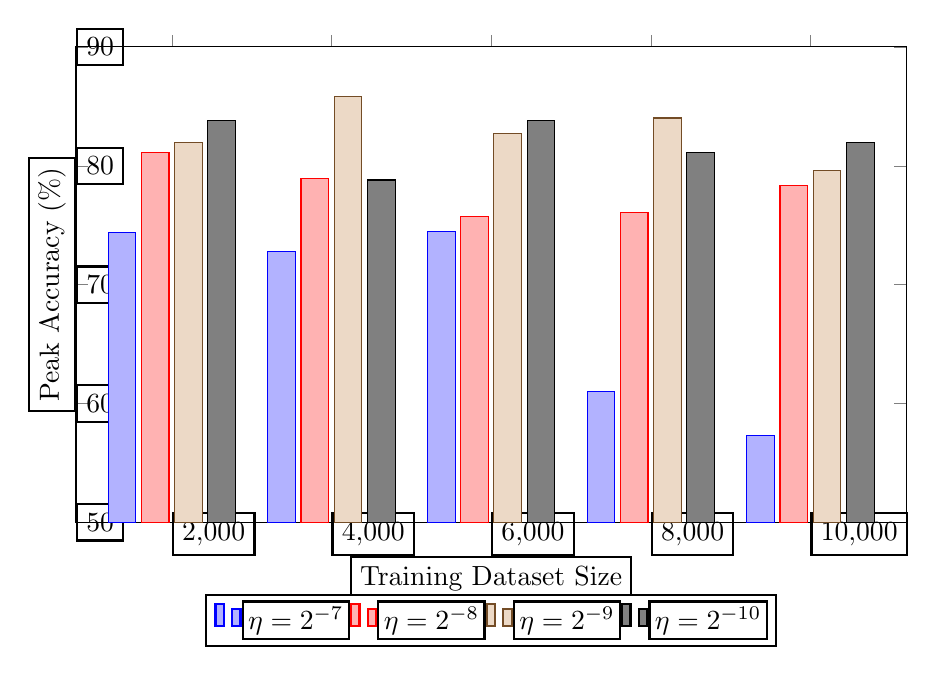
\begin{tikzpicture}
	\begin{axis}[
	ybar,
	height=3in,
	width=\textwidth,
	enlarge y limits=false,
	enlarge x limits=0.15,
	legend style={at={(0.5,-0.15)},
		anchor=north,legend columns=-1},
	ylabel={Peak Accuracy (\%)},
	xlabel={Training Dataset Size},
	ymin=50,
	ymax=90,
	xtick={data},
	scaled y ticks=false,	
	scaled x ticks=false,
	]
	
	\addplot coordinates {(2000, 74.401)  (4000, 72.814) (6000, 74.49) (8000, 61.03) (10000, 57.34)};
	
	\addplot coordinates {(2000, 81.14)  (4000, 78.94) (6000, 75.70) (8000, 76.09) (10000, 78.36)};
	
	\addplot coordinates {(2000, 81.97)  (4000, 85.845) (6000, 82.737) (8000, 84.02) (10000, 79.62)};
	
	\addplot coordinates {(2000, 83.79)  (4000, 78.8) (6000, 83.78) (8000, 81.11) (10000, 81.98)};
	\legend{$\eta = 2^{-7}$, $\eta = 2^{-8}$, $\eta = 2^{-9}$, $\eta = 2^{-10}$}
	\end{axis}
	\end{tikzpicture}
	\caption{Maximum training accuracy reached for various learning rate and training set sizes.}
	\label{training-accuracy}
\end{figure}

\todo[inline]{convergences for swmodel on the network}

\subsection{Stability of Training}
As previously mentioned, due to the relatively low training precision of 18-bit fixed-point, the training process does not converge to a maximum training accuracy, but rather it will reach a maximum training accuracy, and then accuracy will degrade as precision errors accumulate over the training process. Training statistics for the first 10 epochs of the most optimal training configuration from Figure \ref{training-accuracy} illustrate this phenomenon and are shown in Figure \ref{epoch-by-epoch}.

\begin{figure}
	\centering
	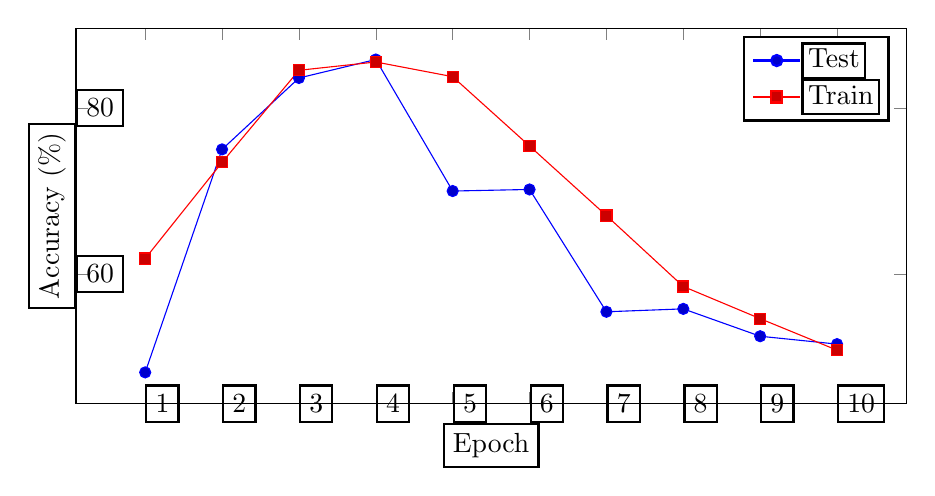
\begin{tikzpicture}
	\begin{axis}[
	ylabel={Accuracy (\%)}, 
	xlabel={Epoch},
	width=\textwidth,
	height=2.5in,
	]
	
	\addplot coordinates 
	{(1, 48.12) (2, 75.012) (3, 83.62) (4, 85.85) (5, 69.99) (6, 70.18) (7, 55.43) (8, 55.78) (9, 52.48) (10, 51.53)};
	\addplot coordinates 	
	{(1, 61.85) (2, 73.45) (3, 84.55) (4, 85.55) (5, 83.78) (6, 75.42) (7, 67.03) (8, 58.48) (9, 54.6) (10, 50.8)};
	
	\legend{Test, Train}
	\end{axis}
	\end{tikzpicture}
	\caption{Epoch-by-epoch training data for an HWM configuration. Clearly visible degradation of accuracy instead of convergence after epoch 4.}
	\label{epoch-by-epoch}
\end{figure}


\section{Implemented Design}
The design implemented for the FPGA is shown in Figure \ref{impl-design}. As expected, the FC1 layer is by and large the most resource intensive, as it utilizes 196 kernels. It is interesting to observe the clustering of individual layer modules, while the interlayer activation buffer for FC0 and FC1 is widely spread out through the FPGA. This would indicate that this interlayer activation buffer was frequently routed to as a midpoint between FC0 and FC1. 

It should be noted that implementation is a non-deterministic process and every design run should result in a slightly different implemented design. However, general trends for routing of the design tend to  persist throughout multiple runs, despite the non-determism of the placing and routing algorithms.

\begin{figure}
	\centering
	\includegraphics[width=\textwidth]{figures/impl_design}
	\includegraphics{figures/impl_design_legend}
	\caption{The implemented design of the hardware model}
	\label{impl-design}
\end{figure}

\subsection{Resource Usage, Power, and Timing}
The resource usage of the hardware model is shown in Table \ref{resource-usage}. As can be seen, the DSP slice is the scarcest resource, with LUTs and BRAMs also heavily being used.  Overall, high utilization of the FPGA resources were made to optimize the performance of the accelerator as much as possible.
\begin{table}
	\centering 
	\begin{tabular}{|l|l|l|c|}
	\hline 
	\textbf{Resource} & \textbf{Utilization} & \textbf{Available} & \textbf{Utilization \%} \\\hline 
	LUT & 41132 & 53200 & 77.32		\\\hline
	FF & 54097 & 106400 & 50.84 \\\hline 
	BRAM & 107.5 & 140 & 76.79 \\\hline 
	DSP & 215 & 220 & 97.73 \\\hline	
	\end{tabular}
\caption{Resource usage of the implemented design}
\label{resource-usage}
\end{table}

According to the Vivado report, the total on-chip power of the design is 2.798 Watts. While this number is reported with `Low' confidence by Vivado, this wattage is far lower than typical GPU power consumptions. Power measurements have not been made for the internal GPU during these experiments, though measurements using the Torch framework were made and reported GPU average power at 94.19 Watts while performing training using the AlexNet architecture.The power measurements were performed with an Nvidia Tesla K20M GPU with 5 GB of GDDR5 SDRAM, a top-of-the-line GPU \cite{xinbochen2016}. This is several magnitudes higher than the FPGA based solution in this thesis. 

The implemented design for the hardware model is clocked at a frequency of 50 MHz. Placement and routing are both able to successfully complete with 0 timing violations. There was no need to improve frequency because the current performance bottleneck of this design stems from data transfer over the AXI bus and not from FPGA computational speed.                                  %Chapter 6
\chapter{Analysis}\label{analysis}

\section{Allocating Computationl Kernels for Performance}
\subsection{Allocating Based on Only Forward Pass Analysis}
When computing an optimal allocation of kernels to the fully-connected layers, it was enough to account only for the forward pass. This is because in the backward pass, there are 2 times the kernel is used, during previous layer neuron gradient calculation, and during weight gradient calculation. In each case, the amount of multiplications is equal to the sum of the fan-ins of all the neurons. For the forward pass, every neuron receives an input from every neuron in the previous layer, so the amount of MACs will be:
\begin{align}
MACs = \text{\#previous layer neurons} \times \text{\#current layer neurons} \label{macs}
\end{align}

For the backward pass, each backpropagated neuron gradient to a previous layer requires an MAC on all the neurons in the current layer. This must be done for each neuron in the previous layer, thus the total amount of MACs for backpropagating neuron gradients is also equivalent to Equation \ref{macs}.

For computing all the weight gradients in a layer, every weight for every neuron must be multiplied by a gradient. Each neuron in the current layer will have a \# previous layer neurons weights, as that is the fan-in for each neuron. Thus, there same amount of multiplications is also equal to the expresion in Equation \ref{macs}.

The backward pass also has a weight updating step, however, this uses bitshifts and not DSP slices to multiply the weight gradient by the learning rate. As such, the backward pass in this model uses exactly twice the amount of multiplications as the forward pass, so the optimal allocation of kernels is optimal for both the forward and backward pass.

\subsection{Allocation Computations}
Table \ref{macs-per-layer} shows the fan-in, number of neurons, and thus the number of MACs per layer during the forward pass.


\section{Cycle Analysis}
\section{Remedies for the Active Cycle Problem}
\section{Granularity in Parallelism}
\section{Balancing Ideal Learning Rate vs. Precision Restrictions}
\section{Remedies for the Lack of Precision}
\subsection{Vanishing Gradient Distribution by Layer}
\subsection{Stability}




                                 	%Chapter 7
\chapter{Discussion}


\section{Main Takeaways of the Thesis}

\section{Future Work}
While the potential for application-specific hardware accelerators training has been demonstrated in this thesis, there is a fair bit of work that would need be done to 

\paragraph{Increased Precision}
As was demonstrated in the results section, training a neural network requires high precision computation. This is especially true for deeper neural networks as a result of the vanishing gradient problem.

\paragraph{Larger Batch Sizes}
Many datasets converge faster using a larger batch size. In addition, a larger batch size provides a more accurate gradient of the actual loss function of the training set. Using a larger batch size would also open up the possibility to taking advantage of data-level parallelism and using an array of training accelerators. 

\paragraph{Additional Layer Types}

\paragraph{Additional Activation Functions}
In both the software and hardware models for this project, the ReLU function was chosen specifically due to its computational simplicity, quick convergence during training, and its ability to frequently converge to a good solution. That being said, there are still many other activation functions in the realm of neural networks that also achieve strong training results. With varying datasets and network architectures, the most optimal activation function may also change. Other functions such as the sigmoid function, leaky ReLU, hyperbolic tangent, and many other could all be more optimal under certain circumstances. These functions would require extra hardware support though, and thus would require more computational resources to implement. As a result, one should expect that the speedup of the accelerator would not be quite so high as with the ReLU activation function.

\paragraph{Implement Streaming DDR Interface for FPGA}

\paragraph{Optimized Algorithms}

\paragraph{Generated HDL for a Pre-Specified Network Architecture}

\paragraph{ASIC Design}
                                 	%Chapter 8
\chapter{Conclusion}\label{conclusion}
This thesis addressed the dearth of performance-optimized solutions for conducting online training of neural networks by proposing a novel hardware architecture. The proposed hardware accelerator achieves high performance by exploiting the fine-grain parallelism present at the neuron level during the training process.

After providing a background of neural networks, a software model was implemented to verify the chosen training algorithm for the hardware model. This provided the algorithmic foundation of the hardware model.

We then provided an explanation of the architecture and implementation of the hardware model. By carefully allocating computational kernels among the fully connected layers, the resultant balanced computational scheme allowed for highly parallelized computation. The implemented design was a modular solution that resulted in a flexible design. Furthermore, full-scale testbenches along with a convenient testing process resulted in the successful verification of the design.

The final design for the hardware accelerator was clocked at 50 MHz and satisfies all timing requirements. Furthermore, the implemented design uses low-power compared to GPUs. Experimental results of the hardware accelerator show that the proposed solution achieves a speedup of 17.35 compared to the next best online training model. At the same time, the accelerator is nearly as fast as the GPU model that performed training with a batch size of 50. The experiments also revealed that the bottleneck of the solution was from the MMIO communication between the PS and FPGA rather than the training on the FPGA. The results also showed that 18 bits of fixed-point precision is not enough to  successfully converge to a local optimum during training, rather the training process will degrade in performance after a few epochs as precision error accumulates. 

We then analyzed and discussed the experimental results, highlighting the need for more computational precision while showing the massive potential gains in performance from utilizing fine-grained parallelism. 

Ultimately, this thesis has shown the feasibility of designing a hardware accelerator that uses neuron-level parallelism for the online training of neural networks. Furthermore, there are many potential future optimizations and improvements that would increase both performance and functionality of the proposed hardware accelerator.                                 	%Chapter 9
\include{Chapter10}                                	%Chapter 10
\appendix
\chapter{Stuff}

\chapter{Stuff2}                                 %Appendix A
%-----------
% Backmatter
%-----------
\backmatter
\chaptermark{Bibliography}
\renewcommand{\sectionmark}[1]{\markright{#1}}
\sectionmark{Bibliography}
\addcontentsline{toc}{chapter}{Bibliography}        %Force addition of Bibliography to TO

\bibliographystyle{alpha}                           %Use alpha codes for references
\bibliography{References}                           %Bibliography file called
\end{document}
% % % EOF % % %